\documentclass[aspectratio=169,12pt]{beamer}
\usepackage[utf8]{inputenc}
\usepackage{amsmath, amssymb}
\usepackage{booktabs}
\usepackage{xcolor}
\usepackage{colortbl}
\usepackage{hyperref}
\usepackage{makecell}
\usepackage{ragged2e}
\usepackage{bytefield}
\usepackage{tikz}
\usetikzlibrary{arrows.meta, positioning, shapes.geometric, calc, tikzmark, shapes.misc, fit, backgrounds}
\usepackage{tcolorbox}
\usetheme{Madrid}

\definecolor{cachecolor}{RGB}{200,220,255}
\definecolor{memcolor}{RGB}{255,220,200}
\definecolor{modifiedcolor}{RGB}{255,200,200}
\definecolor{exclusivecolor}{RGB}{200,255,200}
\definecolor{messageblue}{RGB}{70,130,255}
\definecolor{timecolor}{RGB}{200,100,0}
\definecolor{stateM}{RGB}{200,50,50}
\definecolor{stateE}{RGB}{0,150,0}
\definecolor{stateS}{RGB}{50,50,200}

% Colors for MESI states in diagrams
\definecolor{invalidcolor}{RGB}{255, 200, 100}
\definecolor{sharedcolor}{RGB}{150, 230, 150}
\definecolor{exclusivecolor}{RGB}{150, 200, 255}
\definecolor{modifiedcolor}{RGB}{255, 150, 150}
\definecolor{l2bgcolor}{RGB}{255, 220, 180}
\definecolor{membgcolor}{RGB}{180, 200, 255}

% Ring diagram color palette (cohesive blue-gray theme)
\definecolor{ringSlateBlue}{RGB}{74, 103, 133}      % Main compute die area
\definecolor{ringSteelBlue}{RGB}{107, 140, 174}     % System agent bar
\definecolor{ringGreen}{RGB}{124, 184, 124}         % L2 private cache
\definecolor{ringSand}{RGB}{212, 184, 150}          % LLC shared cache
\definecolor{ringCharcoal}{RGB}{61, 79, 95}         % System components
\definecolor{ringPeach}{RGB}{232, 168, 124}         % iMPH hub
\definecolor{ringLavender}{RGB}{184, 169, 201}      % External I/O
\definecolor{ringCoral}{RGB}{240, 180, 170}         % Polarity marker (odd)
\definecolor{ringCoralLight}{RGB}{255, 220, 210}    % Polarity marker (even)
\definecolor{ringDataPink}{RGB}{220, 150, 200}      % Data message marker

% Macro for the multi-processor example frames
% Arguments: {p1-cache}{p1-state}{p2-cache}{p2-state}{l2-content}{cvb-bits}{memory}
\newcommand{\mpexample}[7]{%
  \centering
  \begin{tikzpicture}[scale=0.7, every node/.style={font=\scriptsize}]
    % L2 Cache - split into two lines
    \node[draw, thick, fill=l2bgcolor, minimum width=4.5cm, minimum height=1cm, align=center] (l2) at (1.5,-2.5) {L2 cache (shared)\\[2pt]#5};

    % Processor 1 box
    \node[draw, thick, fill=green!20, minimum width=2.2cm, minimum height=1.8cm, align=center, anchor=south west] (p1) at ([yshift=20]l2.north west) {};
    \node[above] at (p1.north) {\textbf{Processor 1}};

    % Processor 2 box
    \node[draw, thick, fill=green!20, minimum width=2.2cm, minimum height=1.8cm, align=center, anchor=south east] (p2) at ([yshift=20]l2.north east) {};
    \node[above] at (p2.north) {\textbf{Processor 2}};

    % L1 Caches with content
    \node[draw, thick, fill=lightgray!20, minimum width=1.9cm, minimum height=0.9cm, align=center] (l1p1) at (p1.center) {L1 cache\\[2pt]#1};
    \node[draw, thick, fill=lightgray!20, minimum width=1.9cm, minimum height=0.9cm, align=center] (l1p2) at (p2.center) {L1 cache\\[2pt]#3};

    % State indicators for P1 - positioned at lower right corner
    \ifx&#2&\else
      \ifnum\pdfstrcmp{#2}{M}=0
        \node[circle, draw, thick, fill=orange!70, minimum size=0.4cm, font=\tiny\bfseries] at ($(l1p1.south east)+(-0.15,0.15)$) {M};
      \else\ifnum\pdfstrcmp{#2}{E}=0
        \node[circle, draw, thick, fill=yellow!70, minimum size=0.4cm, font=\tiny\bfseries] at ($(l1p1.south east)+(-0.15,0.15)$) {E};
      \else\ifnum\pdfstrcmp{#2}{S}=0
        \node[circle, draw, thick, fill=cyan!70, minimum size=0.4cm, font=\tiny\bfseries] at ($(l1p1.south east)+(-0.15,0.15)$) {S};
      \else\ifnum\pdfstrcmp{#2}{I}=0
        \node[circle, draw, thick, fill=red!40, minimum size=0.4cm, font=\tiny\bfseries] at ($(l1p1.south east)+(-0.15,0.15)$) {I};
      \fi\fi\fi\fi
    \fi

    % State indicators for P2
    \ifx&#4&\else
      \ifnum\pdfstrcmp{#4}{M}=0
        \node[circle, draw, thick, fill=orange!70, minimum size=0.4cm, font=\tiny\bfseries] at ($(l1p2.south east)+(-0.15,0.15)$) {M};
      \else\ifnum\pdfstrcmp{#4}{E}=0
        \node[circle, draw, thick, fill=yellow!70, minimum size=0.4cm, font=\tiny\bfseries] at ($(l1p2.south east)+(-0.15,0.15)$) {E};
      \else\ifnum\pdfstrcmp{#4}{S}=0
        \node[circle, draw, thick, fill=cyan!70, minimum size=0.4cm, font=\tiny\bfseries] at ($(l1p2.south east)+(-0.15,0.15)$) {S};
      \else\ifnum\pdfstrcmp{#4}{I}=0
        \node[circle, draw, thick, fill=red!40, minimum size=0.4cm, font=\tiny\bfseries] at ($(l1p2.south east)+(-0.15,0.15)$) {I};
      \fi\fi\fi\fi
    \fi

    % Core valid bits
    \node[draw, thick, minimum width=1cm, minimum height=0.6cm, align=center] at ($(l2.east)+(0.9,0)$) {\tiny P1 P2\\[-1pt]#6};

    % Memory
    \node[draw, thick, fill=membgcolor, minimum width=3.8cm, minimum height=0.9cm, align=center, anchor=north] (mem) at ([yshift=-20]l2.south) {Memory\\[2pt]#7};

    % Arrows
    \draw[<->, thick] (p1.south) -- (p1 |- l2.north);
    \draw[<->, thick] (p2.south) -- (p2 |- l2.north);
    \draw[<->, thick] (l2.south) -- (mem.north);
  \end{tikzpicture}
}

\title{MESI Protocol}
\author{Computer Architecture 2360267}
\date{2025, Recitation \#5}
\begin{document}
\frame{\titlepage}

\begin{frame}{Outline}
\tableofcontents
\end{frame}

\section{Cache Coherence Basics}

%==========================================
\begin{frame}{Multi-processor System}
\begin{block}{Memory System Coherence}
A memory system is coherent if:
\end{block}

\begin{enumerate}
\item If P1 writes to address X, and later on, P2 reads X, and there are no other writes to X in between
    \begin{itemize}
    \item[$\Rightarrow$] P2's read returns the value written by P1's write
    \end{itemize}
\item Writes to the same location are serialized:
    \begin{itemize}
    \item Two writes to location X are seen in the same order by all processors
    \end{itemize}
\end{enumerate}

\vspace{1em}
\begin{center}
% Placeholder for processor-cache-memory diagram
\framebox[0.6\textwidth][c]{
\parbox{0.55\textwidth}{\centering
[Diagram: Two processors with L1 caches\\
connected to shared L2 cache and memory]
}}
\end{center}
\end{frame}

%==========================================
\begin{frame}{MESI Protocol States}
Each cache line can be in one of 4 states:

\begin{itemize}
\item \textbf{Invalid (I)} -- Line's data is not valid
\vspace{0.5em}
\item \textbf{Shared (S)} -- Line is valid and not dirty, copies may exist in other processors
\vspace{0.5em}
\item \textbf{Exclusive (E)} -- Line is valid and not dirty, other processors do not have the line in their local caches
\vspace{0.5em}
\item \textbf{Modified (M)} -- Line is valid and dirty, other processors do not have the line in their local caches
\end{itemize}
\end{frame}

%==========================================
\begin{frame}{Multi-processor System: Example (1/3)}
\begin{columns}
\column{0.55\textwidth}
\textbf{Sequence of operations:}
\begin{enumerate}
\item P1 reads address 1000
\item P1 writes address 1000 (value: 5 $\rightarrow$ 6)
\end{enumerate}

\vspace{0.5em}
\textbf{Initial state:} Memory[1000] = 5, both caches empty

\vspace{0.5em}
\textbf{After operations:}
\begin{itemize}
\item P1: \tikz[baseline=-0.5ex]{\node[circle, draw, thick, fill=yellow!70, minimum size=0.4cm, font=\tiny\bfseries] {E};} $\rightarrow$ \tikz[baseline=-0.5ex]{\node[circle, draw, thick, fill=orange!70, minimum size=0.4cm, font=\tiny\bfseries] {M};} (read then write)
\item P2: \tikz[baseline=-0.5ex]{\node[circle, draw, thick, fill=red!40, minimum size=0.4cm, font=\tiny\bfseries] {I};} (still invalid)
\item L2 has stale data (5), Memory unchanged
\end{itemize}

\column{0.45\textwidth}
\mpexample{[1000]: 6}{M}{--}{I}{[1000]: 5}{1~~0}{[1000]: 5}
\end{columns}
\end{frame}

%==========================================
\begin{frame}{Multi-processor System: Example (2/3)}
\begin{columns}
\column{0.55\textwidth}
\textbf{Continuing sequence:}
\begin{enumerate}
\setcounter{enumi}{2}
\item P2 reads address 1000
\end{enumerate}

\vspace{0.5em}
\textbf{What happens:}
\begin{itemize}
\item P2 misses, requests line from L2
\item L2 snoops P1 (CVB shows P1 has it)
\item P1 writes back modified data (6) to L2
\item L2 sends data to P2
\end{itemize}

\vspace{0.5em}
\textbf{Result:}
\begin{itemize}
\item P1: \tikz[baseline=-0.5ex]{\node[circle, draw, thick, fill=orange!70, minimum size=0.4cm, font=\tiny\bfseries] {M};} $\rightarrow$ \tikz[baseline=-0.5ex]{\node[circle, draw, thick, fill=cyan!70, minimum size=0.4cm, font=\tiny\bfseries] {S};}
\item P2: \tikz[baseline=-0.5ex]{\node[circle, draw, thick, fill=red!40, minimum size=0.4cm, font=\tiny\bfseries] {I};} $\rightarrow$ \tikz[baseline=-0.5ex]{\node[circle, draw, thick, fill=cyan!70, minimum size=0.4cm, font=\tiny\bfseries] {S};}
\item Both have value 6
\end{itemize}

\column{0.45\textwidth}
\mpexample{[1000]: 6}{S}{[1000]: 6}{S}{[1000]: 6}{1~~1}{[1000]: 5}
\end{columns}
\end{frame}

%==========================================
\begin{frame}{Multi-processor System: Example (3/3)}
\begin{columns}
\column{0.55\textwidth}
\textbf{Continuing sequence:}
\begin{enumerate}
\setcounter{enumi}{3}
\item P2 requests ownership (RFO) for write intent
\end{enumerate}

\vspace{0.5em}
\textbf{What happens:}
\begin{itemize}
\item P2 sends RFO to L2
\item L2 sends snoop invalidate to P1
\item P1 invalidates its copy
\item L2 grants exclusive ownership to P2
\end{itemize}

\vspace{0.5em}
\textbf{Result:}
\begin{itemize}
\item P1: \tikz[baseline=-0.5ex]{\node[circle, draw, thick, fill=cyan!70, minimum size=0.4cm, font=\tiny\bfseries] {S};} $\rightarrow$ \tikz[baseline=-0.5ex]{\node[circle, draw, thick, fill=red!40, minimum size=0.4cm, font=\tiny\bfseries] {I};}
\item P2: \tikz[baseline=-0.5ex]{\node[circle, draw, thick, fill=cyan!70, minimum size=0.4cm, font=\tiny\bfseries] {S};} $\rightarrow$ \tikz[baseline=-0.5ex]{\node[circle, draw, thick, fill=yellow!70, minimum size=0.4cm, font=\tiny\bfseries] {E};}
\item P2 can now write (E $\rightarrow$ M)
\end{itemize}

\column{0.45\textwidth}
\mpexample{--}{I}{[1000]: 6}{E}{[1000]: 6}{0~~1}{[1000]: 5}
\end{columns}
\end{frame}

%==========================================
\begin{frame}{Core Valid Bits (CVB)}
\begin{block}{What are Core Valid Bits?}
L2 keeps track of the presence of each line in each Core's L1 caches using a bit vector
\end{block}

\vspace{0.5em}
\textbf{Purpose:}
\begin{itemize}
\item Determine if it needs to send a snoop to a processor
\item Determine in what state to provide a requested line (S or E)
\item Track which cores have copies of each cache line
\end{itemize}

\vspace{0.5em}
\textbf{Implementation:}
\begin{itemize}
\item One bit per core for each L2 cache line
\item Bit = 1: Core may have the line in its L1 cache
\item Bit = 0: Core does not have the line in its L1 cache
\end{itemize}

\vspace{0.5em}
\textbf{Example:}
\begin{itemize}
\item CVB = 001: Only Core 0 has the line
\item CVB = 110: Cores 1 and 2 have the line
\item CVB = 000: No core has the line
\end{itemize}
\end{frame}

%==========================================
\begin{frame}{Inclusion Property}
\begin{alertblock}{L2 Cache Inclusion}
The L2 cache must guarantee that all L1 cache lines are included in L2
\end{alertblock}

\vspace{0.5em}
\textbf{Why Inclusion Matters:}
\begin{itemize}
\item Simplifies coherence protocol
\item L2 can track all L1 contents
\item Enables efficient snooping decisions
\end{itemize}

\vspace{0.5em}
\textbf{When L2 Evicts a Line:}
\begin{itemize}
\item L2 must first invalidate the line in all L1 caches
\item L2 sends snoop invalidate to all processors with CVB bit set
\item If line is Modified in L1:
    \begin{itemize}
    \item L1 responds with updated data
    \item L2 writes updated value to memory during eviction
    \end{itemize}
\end{itemize}

\vspace{0.5em}
\textbf{Maintaining Inclusion:}
\begin{itemize}
\item L2 capacity must be larger than sum of L1 caches
\item L2 eviction triggers L1 invalidation
\item Ensures coherence is maintained at L2 level
\end{itemize}
\end{frame}

%==========================================
\begin{frame}{MESI Protocol States -- Summary}
\begin{center}
\begin{tabular}{lccc}
\toprule
State & Valid & Modified & Copies elsewhere?\\
\midrule
\textbf{\textcolor{invalidcolor}{I}}nvalid   & No  & N/A  & possibly\\
\textbf{\textcolor{sharedcolor}{S}}hared    & Yes & No   & possibly\\
\textbf{\textcolor{exclusivecolor}{E}}xclusive & Yes & No   & No\\
\textbf{\textcolor{modifiedcolor}{M}}odified  & Yes & Yes  & No\\
\bottomrule
\end{tabular}
\end{center}

\vspace{1em}
\begin{block}{Write Requires Ownership}
A modified line must be exclusive:
\begin{itemize}
\item Otherwise, another processor with the line will be using stale data
\item To modify, a core must first obtain \textbf{ownership} (no other sharers)
\end{itemize}
\end{block}
\end{frame}

%==========================================
\begin{frame}{MESI Protocol Example - 4 Processors}
\small
Four-processor shared-memory system with MESI protocol

\begin{table}[h]
\centering
\begin{tabular}{|l|c|c|c|c|c|}
\hline
\rowcolor{blue!20}
\textbf{Operation} & \textbf{P0} & \textbf{P1} & \textbf{P2} & \textbf{P3} & \textbf{CVBs} \\
\hline
Initial State & I & I & I & I & 0000 \\
\hline
P0 reads X & E & I & I & I & 1000 \\
\hline
P1 reads X & S & S & I & I & 1100 \\
\hline
P2 reads X & S & S & S & I & 1110 \\
\hline
P3 writes X & I & I & I & M & 0001 \\
\hline
P0 reads X & S & I & I & S & 1001 \\
\hline
\end{tabular}
\end{table}

\textbf{Key observations:}
\begin{itemize}
\item First reader gets Exclusive state (if no other copies exist)
\item Write operation invalidates all other copies
\item Subsequent reads after a write result in Shared state
\end{itemize}
\end{frame}

\section{Question 1: MESI Coherence}

%==========================================
\begin{frame}{MESI Coherence Exercise 1 -- Setup}
\textbf{System Configuration:}
\begin{itemize}
\item 3 Core processor with MESI protocol
\item Each core has an L1 cache, L2 cache is shared (inclusive)
\end{itemize}

\textbf{Message Types:}
\begin{columns}
\column{0.5\textwidth}
\textbf{L1 $\rightarrow$ L2:}
\begin{itemize}
\item Read Address (A)
\item RFO (A) -- Request for Ownership
\item Data (A)
\end{itemize}

\column{0.5\textwidth}
\textbf{L2 $\rightarrow$ L1/Memory:}
\begin{itemize}
\item Read Address (A) to memory
\item Data (A) to L1 with MESI state
\item RFO (A) -- after RFO from L1
\item Snoop (A) to L1
\end{itemize}
\end{columns}

\vspace{1em}
\begin{columns}[t]
\column{0.5\textwidth}
\textbf{Timing:}
\begin{itemize}
\item L1 $\leftrightarrow$ L2: 10ns
\item L2 $\leftrightarrow$ Memory: 100ns
\end{itemize}

\column{0.5\textwidth}
\textbf{CVB (Core Valid Bits):}
\begin{itemize}
\item L2 tracks which cores have each line
\item 1 bit per core per cache line
\end{itemize}
\end{columns}
\end{frame}

%==========================================
% Three-Core MESI Problem - Row by row solution
\newcommand{\mesitwohdr}{%
\footnotesize
\textbf{System:} 3-core MESI, L1 private, L2 shared inclusive\hfill
\textbf{Latencies:} L1$\leftrightarrow$L2: \textcolor{timecolor}{10ns}, L2$\leftrightarrow$Mem: \textcolor{timecolor}{100ns}
\vspace{-3mm}
}

\begin{frame}{MESI Coherence Exercise 1}
\mesitwohdr
\begin{table}[h]
\centering
\renewcommand{\arraystretch}{1.1}
\resizebox{\textwidth}{!}{%
\begin{tabular}{|l|c|c|c|c|c|c|>{\raggedright\arraybackslash}p{7cm}|c|}
\hline
\rowcolor{gray!20}
\textbf{Operation} & \textbf{P1} & \textbf{P2} & \textbf{P3} & \textbf{P1} & \textbf{P2} & \textbf{P3} & \textbf{Messages Sent} & \textbf{Time} \\
\rowcolor{gray!20}
 & \multicolumn{3}{c|}{State} & \multicolumn{3}{c|}{CVB} & & (ns) \\
\hline
Initial & I & I & I & 0 & 0 & 0 & -- & 0 \\
\hline
P2 reads A & \onslide<1->{I} & \onslide<1->{\textcolor{stateE}{\textbf{E}}} & \onslide<1->{I} & \onslide<1->{0} & \onslide<1->{1} & \onslide<1->{0} & \onslide<1->{\vspace{-3mm}\textcolor{messageblue}{L1~miss~$\to$~L2}~\textcolor{timecolor}{(10)}, \textcolor{messageblue}{L2~miss~$\to$~Mem}~\textcolor{timecolor}{(100)}, \textcolor{messageblue}{Mem~$\to$~L2~data}~\textcolor{timecolor}{(100)}, \textcolor{messageblue}{L2~$\to$~L1~data}~\textcolor{timecolor}{(10)}} & \onslide<1->{\textcolor{timecolor}{220}} \\
\hline
P2 writes A & \onslide<2->{I} & \onslide<2->{\textcolor{stateM}{\textbf{M}}} & \onslide<2->{I} & \onslide<2->{0} & \onslide<2->{1} & \onslide<2->{0} & \onslide<2->{\vspace{-3mm}\textcolor{messageblue}{No~messages~(silent~E$\to$M~transition)}} & \onslide<2->{\textcolor{timecolor}{0}} \\
\hline
P1 reads A & \onslide<3->{\textcolor{stateS}{\textbf{S}}} & \onslide<3->{\textcolor{stateS}{\textbf{S}}} & \onslide<3->{I} & \onslide<3->{1} & \onslide<3->{1} & \onslide<3->{0} & \onslide<3->{\vspace{-3mm}\textcolor{messageblue}{L1~miss~$\to$~L2}~\textcolor{timecolor}{(10)}, \textcolor{messageblue}{L2~snoop~$\to$~P2}~\textcolor{timecolor}{(10)}, \textcolor{messageblue}{P2~data~$\to$~L2}~\textcolor{timecolor}{(10)}, \textcolor{messageblue}{L2~data~$\to$~P1}~\textcolor{timecolor}{(10)}} & \onslide<3->{\textcolor{timecolor}{40}} \\
\hline
P2 reads A & \onslide<4->{\textcolor{stateS}{\textbf{S}}} & \onslide<4->{\textcolor{stateS}{\textbf{S}}} & \onslide<4->{I} & \onslide<4->{1} & \onslide<4->{1} & \onslide<4->{0} & \onslide<4->{\vspace{-3mm}\textcolor{messageblue}{Cache~hit~--~no~messages}} & \onslide<4->{\textcolor{timecolor}{0}} \\
\hline
P3 reads A & \onslide<5->{\textcolor{stateS}{\textbf{S}}} & \onslide<5->{\textcolor{stateS}{\textbf{S}}} & \onslide<5->{\textcolor{stateS}{\textbf{S}}} & \onslide<5->{1} & \onslide<5->{1} & \onslide<5->{1} & \onslide<5->{\vspace{-3mm}\textcolor{messageblue}{L1~miss~$\to$~L2}~\textcolor{timecolor}{(10)}, \textcolor{messageblue}{L2~hit~$\to$~P3~data}~\textcolor{timecolor}{(10)}} & \onslide<5->{\textcolor{timecolor}{20}} \\
\hline
P3 writes A & \onslide<6->{I} & \onslide<6->{I} & \onslide<6->{\textcolor{stateM}{\textbf{M}}} & \onslide<6->{0} & \onslide<6->{0} & \onslide<6->{1} & \onslide<6->{\vspace{-3mm}\textcolor{messageblue}{RFO~$\to$~L2}~\textcolor{timecolor}{(10)}, \textcolor{messageblue}{L2~snoop~inv~P1+P2}~\textcolor{timecolor}{(10)}, \textcolor{messageblue}{L2~$\to$~P3~grant}~\textcolor{timecolor}{(10)}} & \onslide<6->{\textcolor{timecolor}{30}} \\
\hline
\end{tabular}
}
\end{table}

\begin{tcolorbox}[colback=green!5, colframe=green!50!black, top=1mm, bottom=1mm]
\footnotesize
\only<1>{Cold miss $\Rightarrow$ full memory round-trip. \textbf{E} state since P2 is the only holder.}%
\only<2>{\textbf{E$\to$M is free!} Silent transition, no bus traffic. Key advantage of Exclusive state.}%
\only<3>{P2 has Modified $\Rightarrow$ L2 snoops, P2 returns dirty data. Both become \textbf{S}.}%
\only<4>{L1 cache hit! Data served directly, no bus traffic.}%
\only<5>{L2 hit on clean data $\Rightarrow$ no snoop needed. All three now in \textbf{S}.}%
\only<6>{S$\to$M requires RFO $\Rightarrow$ L2 invalidates P1+P2. P3 gets exclusive ownership.}%
\end{tcolorbox}
\end{frame}

\section{Protocol Mechanisms}

%==========================================
\begin{frame}{Read For Ownership (RFO)}
\begin{block}{RFO Request}
A signal from private to shared cache (L1$\rightarrow$L2) requesting cache line exclusivity for write intent
\end{block}

\textbf{RFO Process:}
\begin{enumerate}
\item L1 sends RFO to L2/LLC
\item MLC/LLC invalidates cache line in other L1s
\item MLC/LLC responds to L1 that RFO has been granted
\item L1 can now modify cache line
\end{enumerate}

\vspace{1em}
\begin{alertblock}{RFO Guarantees Coherence}
RFO ensures exclusive access before modification, maintaining cache coherence
\end{alertblock}
\end{frame}

%==========================================
\begin{frame}{Global Observation (GO)}
\begin{block}{Global Observation}
L2 sends a notification to all processors before delivering the actual data to the requesting L1 cache. This notification informs all processors that a specific cache line is being accessed.
\end{block}

\textbf{The Global Observation message indicates the MESI state (E or S) for the requested line}

\vspace{0.2em}
\textbf{Two-step L1$\rightarrow$L2 line request:}
\begin{enumerate}
\item \textbf{GO} - Global Observation with MESI state
\item \textbf{Fill} - Actual data transfer
\end{enumerate}

\vspace{0.2em}
\begin{alertblock}{GO and Fill Timing}
GO and data may be sent at different cycles:
\vspace{-0.3em}
\begin{columns}
\column{0.5\textwidth}
\begin{itemize}
\item GO is the outcome of a tag-hit
\end{itemize}
\column{0.5\textwidth}
\begin{itemize}
\item Data comes from the data array
\end{itemize}
\end{columns}
\end{alertblock}
\end{frame}

\section{Question 2: MESI Coherence}

%==========================================
\begin{frame}{MESI Coherence Exercise 2 -- Setup}
\footnotesize
\textbf{System Configuration:}
\begin{itemize}
\item 2 processors (P0 and P1) with MESI protocol
\item Each processor has L1 cache, shared L2 cache (inclusive)
\item Direct-mapped caches with write allocate + write back
\end{itemize}

\textbf{Latencies:}
\begin{itemize}
\item L1 access: 3ns
\item L1 $\leftrightarrow$ L2 message: 20ns
\item L2 $\leftrightarrow$ Memory message: 90ns
\end{itemize}

\textbf{Important Details:}
\begin{itemize}
\item Parallel messages possible on different channels
\item X1-X5 are separate cache lines
\item X1-X4 map to same L1 set, X5 to different L1 set
\item X1-X2 map to same L2 set, X3-X5 to different L2 set
\end{itemize}

\vspace{0.5em}
\begin{tcolorbox}[colback=blue!5, colframe=blue!50, fonttitle=\footnotesize, title=Exercise]
For each operation, determine: messages sent, time taken, CVB values, and final MESI state.
\end{tcolorbox}
\end{frame}

%==========================================
% MESI Coherence Problem - Row by row solution
\newcommand{\mesicellvs}{-3mm}
\begin{frame}{MESI Coherence Exercise 2}
\scriptsize
\begin{columns}[t]
\column{0.5\textwidth}
\textbf{System:} 2 proc, MESI, L1 priv, L2 shared incl, direct-map\\
\textbf{Latencies:} L1: \textcolor{timecolor}{3ns}, L1$\leftrightarrow$L2: \textcolor{timecolor}{20ns}, L2$\leftrightarrow$Mem: \textcolor{timecolor}{90ns}
\column{0.5\textwidth}
\textbf{L1 Mapping:} X1,X2,X3,X4 $\to$ same set; X5 $\to$ different set\\
\textbf{L2 Mapping:} X1,X2 $\to$ same set; X3,X4,X5 $\to$ different sets
\end{columns}
\tiny
\vspace{-1mm}
\begin{table}[h]
\centering
\setlength{\tabcolsep}{1pt}
\renewcommand{\arraystretch}{1.2}
\resizebox{\textwidth}{!}{%
\begin{tabular}{|c|l|c|c|c|c|>{\raggedright\arraybackslash}p{9cm}|c|}
\hline
\rowcolor{gray!20}
\# & \textbf{Operation} & \textbf{P0} & \textbf{P1} & \textbf{P0} & \textbf{P1} & \textbf{Messages Sent} & \textbf{Time} \\
\rowcolor{gray!20}
 & & \multicolumn{2}{c|}{State} & \multicolumn{2}{c|}{CVB} & & (ns) \\
\hline
1 & \makecell[l]{P0\\reads X1} & \onslide<2->{\textcolor{stateE}{\textbf{E}}} & \onslide<2->{I} & \onslide<2->{1} & \onslide<2->{0} & \onslide<2->{\vspace{\mesicellvs}\textcolor{messageblue}{P0~$\to$~L1~miss}~\textcolor{timecolor}{(3)}, \textcolor{messageblue}{L1~$\to$~L2~rd~miss}~\textcolor{timecolor}{(20)}, \textcolor{messageblue}{L2~$\to$~MEM~rd}~\textcolor{timecolor}{(90)}, \textcolor{messageblue}{MEM~$\to$~L2~data}~\textcolor{timecolor}{(90)}, \textcolor{messageblue}{L2~$\to$~L1~data}~\textcolor{timecolor}{(20)}, \textcolor{messageblue}{L1~$\to$~P0~data}~\textcolor{timecolor}{(3)}} & \onslide<2->{\textcolor{timecolor}{226}} \\
\hline
2 & \makecell[l]{P1\\writes X3} & I & \textcolor{stateM}{\textbf{M}} & 0 & 1 & \vspace{\mesicellvs}\textcolor{messageblue}{P1~$\to$~L1~miss}~\textcolor{timecolor}{(3)}, \textcolor{messageblue}{L1~$\to$~L2~rd~miss}~\textcolor{timecolor}{(20)}, \textcolor{messageblue}{L2~$\to$~MEM~rd}~\textcolor{timecolor}{(90)}, \textcolor{messageblue}{MEM~$\to$~L2~data}~\textcolor{timecolor}{(90)}, \textcolor{messageblue}{L2~$\to$~L1~data}~\textcolor{timecolor}{(20)}, \textcolor{messageblue}{L1~$\to$~P1~write}~\textcolor{timecolor}{(3)} & \textcolor{timecolor}{226} \\
\hline
3 & \makecell[l]{P1\\writes X4} & \onslide<3->{I} & \onslide<3->{\textcolor{stateM}{\textbf{M}}} & \onslide<3->{0} & \onslide<3->{1} & \onslide<3->{\vspace{\mesicellvs}\textcolor{messageblue}{P1~$\to$~L1~miss}~\textcolor{timecolor}{(3)}, \textcolor{messageblue}{L1~$\to$~L2~wb}~\textcolor{timecolor}{(20)}, \textcolor{messageblue}{L1~$\to$~L2~rd~miss}~\textcolor{timecolor}{(20)}, \textcolor{messageblue}{L2~$\to$~MEM~wb}~\textcolor{timecolor}{(90)}, \textcolor{messageblue}{L2~$\to$~MEM~rd}~\textcolor{timecolor}{(90)}, \textcolor{messageblue}{MEM~$\to$~L2~data}~\textcolor{timecolor}{(90)}, \textcolor{messageblue}{L2~$\to$~L1~data}~\textcolor{timecolor}{(20)}, \textcolor{messageblue}{L1~$\to$~P1~write}~\textcolor{timecolor}{(3)}} & \onslide<3->{\textcolor{timecolor}{336}} \\
\hline
4 & \makecell[l]{P1\\writes X5} & \onslide<4->{I} & \onslide<4->{\textcolor{stateM}{\textbf{M}}} & \onslide<4->{0} & \onslide<4->{1} & \onslide<4->{\vspace{\mesicellvs}\textcolor{messageblue}{P1~$\to$~L1~miss}~\textcolor{timecolor}{(3)}, \textcolor{messageblue}{L1~$\to$~L2~rd~miss}~\textcolor{timecolor}{(20)}, \textcolor{messageblue}{L2~$\to$~L1~snoop}~\textcolor{timecolor}{(20)}, \textcolor{messageblue}{L1~$\to$~L2~data}~\textcolor{timecolor}{(20)}, \textcolor{messageblue}{L2~$\to$~MEM~wb}~\textcolor{timecolor}{(90)}, \textcolor{messageblue}{L2~$\to$~MEM~rd}~\textcolor{timecolor}{(90)}, \textcolor{messageblue}{MEM~$\to$~L2~data}~\textcolor{timecolor}{(90)}, \textcolor{messageblue}{L2~$\to$~L1~data}~\textcolor{timecolor}{(20)}, \textcolor{messageblue}{L1~$\to$~P1~write}~\textcolor{timecolor}{(3)}} & \onslide<4->{\textcolor{timecolor}{356}} \\
\hline
5 & \makecell[l]{P0\\reads X5} & \onslide<5->{\textcolor{stateS}{\textbf{S}}} & \onslide<5->{\textcolor{stateS}{\textbf{S}}} & \onslide<5->{1} & \onslide<5->{1} & \onslide<5->{\vspace{\mesicellvs}\textcolor{messageblue}{P0~$\to$~L1~miss}~\textcolor{timecolor}{(3)}, \textcolor{messageblue}{L1~$\to$~L2~rd~miss}~\textcolor{timecolor}{(20)}, \textcolor{messageblue}{L2~$\to$~P1~snoop}~\textcolor{timecolor}{(20)}, \textcolor{messageblue}{P1~$\to$~L2~data}~\textcolor{timecolor}{(20)}, \textcolor{messageblue}{L2~$\to$~L1~data}~\textcolor{timecolor}{(20)}, \textcolor{messageblue}{L1~$\to$~P0~data}~\textcolor{timecolor}{(3)}} & \onslide<5->{\textcolor{timecolor}{86}} \\
\hline
6 & \makecell[l]{P1\\reads X4} & \onslide<6->{I} & \onslide<6->{\textcolor{stateE}{\textbf{E}}} & \onslide<6->{0} & \onslide<6->{1} & \onslide<6->{\vspace{\mesicellvs}\textcolor{messageblue}{P1~$\to$~L1~miss}~\textcolor{timecolor}{(3)}, \textcolor{messageblue}{L1~$\to$~L2~rd~miss}~\textcolor{timecolor}{(20)}, \textcolor{messageblue}{\{L2~snoop~P0+P1~+~L2~$\to$~MEM~wb\}}~\textcolor{timecolor}{(90)}, \textcolor{messageblue}{L2~$\to$~MEM~rd}~\textcolor{timecolor}{(90)}, \textcolor{messageblue}{MEM~$\to$~L2~data}~\textcolor{timecolor}{(90)}, \textcolor{messageblue}{L2~$\to$~L1~data}~\textcolor{timecolor}{(20)}, \textcolor{messageblue}{L1~$\to$~P1~data}~\textcolor{timecolor}{(3)}} & \onslide<6->{\textcolor{timecolor}{316}} \\
\hline
\end{tabular}
}
\end{table}

\begin{tcolorbox}[colback=green!5, colframe=green!50!black, top=1mm, bottom=1mm]
\footnotesize
\only<1>{\textbf{Given:} Row 2 result. Work backwards to understand row 1, then forward for rows 3--6.}%
\only<2>{Cold miss $\Rightarrow$ full memory round-trip. \textbf{E} state since P0 is the only holder.}%
\only<3>{X3/X4 same L1 set $\Rightarrow$ evict X3 (Modified $\Rightarrow$ writeback).}%
\only<4>{L2 miss $\Rightarrow$ \textbf{Inclusion}: L2 snoops P1 for X4 (modified), gets writeback.}%
\only<5>{L2 hit but P1 has X5 Modified $\Rightarrow$ snoop gets dirty data. Both become \textbf{S}.}%
\only<6>{L1+L2 miss $\Rightarrow$ fetch from memory. X5 evicted from L2 $\Rightarrow$ snoop+writeback. \{braces\} = parallel.}%
\end{tcolorbox}
\end{frame}


\section{Ring Interconnect}

%==========================================
\begin{frame}{Ring Interconnect}
\begin{center}
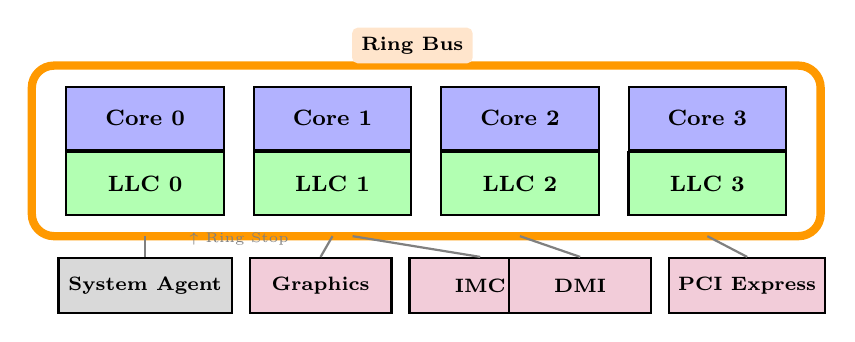
\begin{tikzpicture}[
    scale=0.85,
    % Node styles
    core/.style={rectangle, draw, thick, fill=blue!30, minimum width=2cm, minimum height=0.8cm, font=\footnotesize\bfseries},
    llc/.style={rectangle, draw, thick, fill=green!30, minimum width=2cm, minimum height=0.8cm, font=\footnotesize\bfseries},
    sysagent/.style={rectangle, draw, thick, fill=gray!30, minimum width=2.2cm, minimum height=0.7cm, font=\scriptsize\bfseries},
    peripheral/.style={rectangle, draw, thick, fill=purple!20, minimum width=1.8cm, minimum height=0.7cm, font=\scriptsize\bfseries},
    ring/.style={line width=3pt, orange!80!yellow},
]

% Core + LLC blocks (using relative positioning)
\node[core] (core0) at (0, 0) {Core 0};
\node[llc, below=0pt of core0] (llc0) {LLC 0};

\node[core] (core1) at (2.8, 0) {Core 1};
\node[llc, below=0pt of core1] (llc1) {LLC 1};

\node[core] (core2) at (5.6, 0) {Core 2};
\node[llc, below=0pt of core2] (llc2) {LLC 2};

\node[core] (core3) at (8.4, 0) {Core 3};
\node[llc, below=0pt of core3] (llc3) {LLC 3};

% Ring path coordinates
\coordinate (ring-tl) at ([xshift=-0.5cm, yshift=0.3cm]core0.north west);
\coordinate (ring-tr) at ([xshift=0.5cm, yshift=0.3cm]core3.north east);
\coordinate (ring-bl) at ([xshift=-0.5cm, yshift=-0.3cm]llc0.south west);
\coordinate (ring-br) at ([xshift=0.5cm, yshift=-0.3cm]llc3.south east);

% Draw ring (rectangular path)
\draw[ring, rounded corners=8pt]
    (ring-tl) -- (ring-tr) -- (ring-br) -- (ring-bl) -- cycle;

% Ring label
\node[fill=orange!20, font=\scriptsize\bfseries, rounded corners=2pt] at ([yshift=0.6cm]core1.north east) {Ring Bus};

% Bottom components - System Agent side (left)
\node[sysagent] (sa) at (0, -2.5) {System Agent};
\node[peripheral, right=0.2cm of sa] (gfx) {Graphics};
\node[peripheral, right=0.2cm of gfx] (imc) {IMC};

% Bottom components - I/O side (right)
\node[peripheral] (dmi) at (6.5, -2.5) {DMI};
\node[peripheral, right=0.2cm of dmi] (pcie) {PCI Express};

% Connections from ring to bottom components
\draw[thick, gray] ([yshift=-0.3cm]llc0.south) -- (sa.north);
\draw[thick, gray] ([yshift=-0.3cm]llc1.south) -- (gfx.north);
\draw[thick, gray] ([yshift=-0.3cm, xshift=0.3cm]llc1.south) -- (imc.north);
\draw[thick, gray] ([yshift=-0.3cm]llc2.south) -- (dmi.north);
\draw[thick, gray] ([yshift=-0.3cm]llc3.south) -- (pcie.north);

% Labels for ring connections
\node[font=\tiny, text=gray] at (1.4, -1.8) {$\uparrow$ Ring Stop};

\end{tikzpicture}
\end{center}

\vspace{-0.3cm}
\begin{columns}[T]
\column{0.5\textwidth}
\footnotesize
\textbf{Ring Components:}
\begin{itemize}
\item 4 Core/LLC slices as ring stops
\item Bidirectional ring for data transfer
\end{itemize}

\column{0.5\textwidth}
\footnotesize
\textbf{Connected Agents:}
\begin{itemize}
\item System Agent, Graphics, IMC (memory)
\item DMI (chipset), PCIe (expansion)
\end{itemize}
\end{columns}
\end{frame}

%==========================================
\begin{frame}{Ring Architecture Details}
\textbf{Ring Configuration:}
\begin{itemize}
\item 2 × 4 rings: Req / Data / Ack / Snoop
\item Packets always use the shortest path
\item Static Even/Odd polarity per station
\item Each ring switches polarity on each cycle --- simplifies arbitration at each stop
\end{itemize}

\vspace{1em}
\begin{block}{Polarity-Based Flow Control}
A stop can only pull data from the direction (ring) that matches its polarity in the current cycle
\begin{itemize}
\item[$\Rightarrow$] Sender must ensure data can be pulled by receiver when it arrives
\end{itemize}
\end{block}

\textbf{Example Configuration:}
\begin{itemize}
\item 64B cache line (L1/L2/LLC)
\item 32B/cycle bus bandwidth
\item[$\Rightarrow$] Cache line transfers from LLC to L1 in two strokes
\end{itemize}
\end{frame}

%==========================================
\begin{frame}{Ring Example - Data Transfer}
\footnotesize
\textbf{Scenario:} Core 0, Core 1, and GFX issue data read requests

\vspace{0.5em}
\begin{center}
% Placeholder for ring timing diagram
\framebox[0.9\textwidth][c]{
\parbox{0.85\textwidth}{\centering
[Timing Diagram: Ring cycles 1-15\\
Shows Request, Global Observation, and Data phases\\
Even/Odd polarity switching per cycle]
}}
\end{center}

\vspace{0.5em}
\textbf{Key Events:}
\begin{enumerate}
\item GFX request delayed (odd distance, must arrive on Even cycle)
\item Both Core requests hit in LLC, CVBs indicate no snoop needed
\item LLC sends first chunk (1/2 cache line) to each core
\item LLC sends GO with MESI state (E/S)
\item LLC sends second chunk to complete transfer
\end{enumerate}
\end{frame}

%==========================================
% Ring Example - Data Transfer Animation
\begin{frame}{Ring Example -- Data Transfer}
% Top explanation - plain text above the diagram
\only<1>{\textbf{Initial State:} Ring connects all agents. Each stop has Odd/Even polarity.}%
\only<2>{Core 0, Core 1 and the GFX issue data read requests}%
\only<3>{Requests travel on ring. GFX delayed: odd polarity, must wait for Even cycle}%
\only<4>{Both Core requests hit in LLC. CVBs show no snoop needed}%
\only<5>{GFX request arrives at LLC1}%
\only<6>{LLC sends GO (Global Observation) with MESI state to cores}%
\only<7>{LLC sends first data chunk (D1 = 32B, half cache line)}%
\only<8>{LLC sends second chunk (D2). GFX receives GO.}%
\only<9>{All cores received full cache line. Transfer complete.}%
\vspace{1mm}
\centering
\begin{tikzpicture}[
    scale=0.78,
    every node/.style={font=\small},
    % Base style for all system agent components
    sysbase/.style={draw=black, thick, minimum height=0.85cm, font=\small\bfseries},
    % L2 box - soft green for private cache
    l2box/.style={draw=black, thick, fill=ringGreen, minimum width=1.2cm, minimum height=0.8cm, font=\normalsize\bfseries},
    % LLC box - warm sand for shared cache
    llcbox/.style={draw=black, thick, fill=ringSand, minimum width=1.8cm, minimum height=1.4cm, font=\normalsize\bfseries},
    % System agent components - charcoal with white text
    sysbox/.style={sysbase, fill=ringCharcoal, minimum width=1.4cm, text=white},
    % iMPH - peach accent (the ring hub)
    imphbox/.style={sysbase, fill=ringPeach, minimum width=2.0cm, minimum height=1.0cm, font=\normalsize\bfseries},
    % External IO/DDR - lavender for off-die
    extbox/.style={draw=black, thick, fill=ringLavender, minimum width=1.1cm, minimum height=4.0cm, font=\Large\bfseries},
    % Polarity markers - coral/salmon tones visible on blue
    polaritymark/.style={circle, draw=white, line width=1.5pt, minimum size=0.6cm, font=\normalsize\bfseries, text=black},
    pOdd/.style={polaritymark, fill=ringCoral},
    pEven/.style={polaritymark, fill=ringCoralLight},
    % Ring arrows - white on blue background
    ringarrow/.style={-{Triangle[width=7pt,length=6pt]}, line width=3.5pt, white},
    % Message markers - semantic colors
    request/.style={circle, draw=red!80, very thick, fill=red!65, minimum size=0.65cm, font=\tiny\bfseries, text=white, align=center},
    gomark/.style={circle, draw=gray!70, very thick, fill=gray!50, minimum size=0.6cm, font=\tiny\bfseries, align=center},
    datamark/.style={circle, draw=magenta!60, very thick, fill=ringDataPink, minimum size=0.6cm, font=\tiny\bfseries, align=center},
    % Callout style
    callout/.style={draw=black!60, fill=white, rounded corners=2pt, font=\scriptsize, align=left, inner sep=3pt},
]

% === MAIN BLUE CONTAINER (slate blue) ===
\fill[ringSlateBlue, rounded corners=2pt] (-0.3, -4.6) rectangle (9.3, 2.0);

% === SYSTEM AGENT BAR (steel blue - lighter) ===
\fill[ringSteelBlue] (-0.3, 1.1) rectangle (9.3, 2.0);
\node[font=\scriptsize\bfseries, text=white, align=center] at (0.7, 1.55) {System\\Agent};
\node[sysbox] (ncu) at (2.0, 1.55) {NCU};
\node[font=\scriptsize, text=white] at (2.0, 0.95) {PEG/DMI};
\node[imphbox] (imph) at (4.5, 1.5) {iMPH};
\node[sysbox, minimum width=1.6cm] (mc) at (7.2, 1.55) {MC};

% === ROW SEPARATORS ===
\draw[black, line width=1.2pt] (-0.3, 1.1) -- (9.3, 1.1);
\draw[black, line width=1.2pt] (-0.3, -0.5) -- (9.3, -0.5);
\draw[black, line width=1.2pt] (-0.3, -2.5) -- (9.3, -2.5);

% === CORE 0 ROW ===
\node[font=\large\bfseries, text=white] at (0.8, 0.3) {Core 0};
\node[l2box] (l2c0) at (2.2, 0.3) {L2};
\node[llcbox] (llc0) at (8.0, 0.3) {LLC0};

% === CORE 1 ROW ===
\node[font=\large\bfseries, text=white] at (0.8, -1.5) {Core 1};
\node[l2box] (l2c1) at (2.2, -1.5) {L2};
\node[llcbox] (llc1) at (8.0, -1.5) {LLC1};

% === GFX ROW ===
\node[font=\large\bfseries, text=white] at (0.8, -3.55) {GFX};
\node[l2box] (l2gfx) at (2.2, -3.55) {};

% === RING STRUCTURE ===
% Ring connection point from iMPH
\node[pOdd, fill=pink!50] (imphring) at (4.5, 0.75) {};
\draw[ringarrow] (imph.south) -- (imphring.north);

% Left column (down ring) - polarity markers with labels
\node[pOdd] (ring0l) at (3.8, 0.3) {O};
\node[pEven] (ring1l) at (3.8, -1.5) {e};
\node[pOdd] (ring2l) at (3.8, -3.55) {O};

% Right column (up ring) - polarity matches row (same as left column)
\node[pOdd] (ring0r) at (5.8, 0.3) {O};
\node[pEven] (ring1r) at (5.8, -1.5) {e};
\node[pOdd] (ring2r) at (5.8, -3.55) {O};

% Up ring arrows (left column, going up)
\draw[ringarrow] (ring2l.north) -- (ring1l.south);
\draw[ringarrow] (ring1l.north) -- (ring0l.south);
\draw[ringarrow] (ring0l.north) -- ++(-0.3, 0.15) -- (imphring.south west);

% Down ring arrows (right column, going down)
\draw[ringarrow] (imphring.south east) -- ++(0.3,-0.15) -- (ring0r.north);
\draw[ringarrow] (ring0r.south) -- (ring1r.north);
\draw[ringarrow] (ring1r.south) -- (ring2r.north);

% Bottom connection between left and right columns (right to left)
\coordinate (ringbottom) at (4.8, -4.25);
\draw[ringarrow] (ring2r.south) |- (ringbottom) -| (ring2l.south);

% === EXTERNAL: IO (left) ===
\node[extbox] (io) at (-1.4, -1.3) {IO};
\draw[{Triangle[width=7pt,length=6pt]}-, line width=3.5pt, green!50!black] ([yshift=6pt]io.east) -- ++(0.5, 0);
\draw[-{Triangle[width=7pt,length=6pt]}, line width=3.5pt, green!50!black] ([yshift=-6pt]io.east) -- ++(0.5, 0);

% === EXTERNAL: DDR (right) ===
\node[extbox] (ddr) at (10.5, -1.3) {DDR};
\draw[{Triangle[width=7pt,length=6pt]}-, line width=3.5pt, green!50!black] ([yshift=6pt]ddr.west) -- ++(-0.5, 0);
\draw[-{Triangle[width=7pt,length=6pt]}, line width=3.5pt, green!50!black] ([yshift=-6pt]ddr.west) -- ++(-0.5, 0);

% === LEGEND (left side) - marker sample + label ===
% Legend box background
\node[draw=black, fill=white, rounded corners=3pt, minimum width=1.6cm, minimum height=2.2cm, anchor=north] (legendbg) at (-1.4, 1.9) {};
% Marker samples with labels
\node[circle, draw=red!80, very thick, fill=red!60, minimum size=0.4cm] (legReq) at (-1.75, 1.55) {};
\node[font=\scriptsize, anchor=west] at (-1.5, 1.55) {Request};
\node[circle, draw=gray!60, very thick, fill=gray!45, minimum size=0.4cm] (legGO) at (-1.75, 1.0) {};
\node[font=\scriptsize, anchor=west] at (-1.5, 1.0) {GO};
\node[circle, draw=magenta!70, very thick, fill=magenta!35, minimum size=0.4cm] (legData) at (-1.75, 0.45) {};
\node[font=\scriptsize, anchor=west] at (-1.5, 0.45) {Data};

% === CYCLE INDICATOR (bottom) ===
\node[font=\normalsize\bfseries] at (4.5, -5.0) {%
    \only<1>{Initial state}%
    \only<2>{Cycle 1: up ring E, down ring O}%
    \only<3>{Cycle 2: up ring O, down ring E}%
    \only<4>{Cycle 3: up ring E, down ring O}%
    \only<5>{Cycle 4: up ring O, down ring E}%
    \only<6>{Cycle 5: up ring E, down ring O}%
    \only<7>{Cycle 7: up ring E, down ring O}%
    \only<8>{Cycle 9: up ring E, down ring O}%
    \only<9>{Cycle 11: up ring E, down ring O}%
};

% === SLIDE 1: Initial state with callouts ===
\only<1>{
    % --- LEFT SIDE CALLOUTS ---
    % Callout for Odd polarity - points to ring0l (O)
    \node[callout] (calloutOdd) at (-2.8, 0.3) {\textbf{O} = Odd polarity};
    \draw[->, black!60, thick] (calloutOdd.east) -- (ring0l.west);

    % Callout for Even polarity - points to ring1l (e)
    \node[callout] (calloutEven) at (-2.8, -1.5) {\textbf{e} = Even polarity};
    \draw[->, black!60, thick] (calloutEven.east) -- (ring1l.west);

    % --- RIGHT SIDE CALLOUTS (system components) ---
    % iMPH callout
    \node[callout, anchor=west] (calloutIMPH) at (10.0, 1.5) {%
        \textbf{iMPH}: Memory Protocol Hub\\
        Ring interconnect hub};
    \draw[->, black!60, thick] (calloutIMPH.west) -- (imph.east);

    % MC callout
    \node[callout, anchor=west] (calloutMC) at (10.0, 0.5) {%
        \textbf{MC}: Memory Controller\\
        Interfaces with DDR};
    \draw[->, black!60, thick] (calloutMC.west) -| ([xshift=3pt]mc.east);

    % NCU callout (left side, above IO)
    \node[callout, anchor=east] (calloutNCU) at (-2.8, 1.5) {%
        \textbf{NCU}: Non-Core Unit\\
        System functions};
    \draw[->, black!60, thick] (calloutNCU.east) -- (ncu.west);

    % PEG/DMI note
    \node[callout, anchor=east] (calloutPEG) at (-2.8, -2.8) {%
        \textbf{PEG}: PCIe Graphics\\
        \textbf{DMI}: Direct Media I/F};
    \draw[->, black!60, thick] (calloutPEG.north east) -- (2.0, 0.95);

    % Note about alternation
    \node[font=\scriptsize, text=white] at (4.8, -4.6) {Polarity alternates each ring cycle};
}

% === CYCLE 2: Requests issued ===
\only<2>{
    \node[request] at ([xshift=14pt]l2c0.east) {DRd\\[-1pt]0$\to$1};
    \node[request] at ([xshift=14pt]l2c1.east) {DRd\\[-1pt]1$\to$0};
    \node[request] at ([xshift=14pt]l2gfx.east) {DRd\\[-1pt]G$\to$1};
}

% === CYCLE 3: Requests moving ===
\only<3>{
    \node[request] at ([xshift=12pt]ring0r.east) {DRd\\[-1pt]0$\to$1};
    \node[request] at ([xshift=-12pt]ring1l.west) {DRd\\[-1pt]1$\to$0};
    \node[request] at ([xshift=14pt]l2gfx.east) {DRd\\[-1pt]G$\to$1};
}

% === CYCLE 4: LLC hits ===
\only<4>{
    \node[request] at ([xshift=-12pt]ring1l.west) {DRd\\[-1pt]G$\to$1};
    \node[font=\scriptsize\bfseries, fill=yellow!80, draw=red!70, rounded corners=2pt, inner sep=2pt] at ([xshift=-20pt]llc0.west) {Hit};
    \node[font=\scriptsize\bfseries, fill=yellow!80, draw=red!70, rounded corners=2pt, inner sep=2pt] at ([xshift=-20pt]llc1.west) {Hit};
}

% === CYCLE 5: GFX arrives ===
\only<5>{
    \node[request] at ([xshift=-12pt]llc1.west) {DRd\\[-1pt]G$\to$1};
}

% === CYCLE 6: GO sent ===
\only<6>{
    \node[gomark] at ([xshift=-12pt]ring0l.west) {GO\\[-1pt]1};
    \node[gomark] at ([xshift=12pt]ring1r.east) {GO\\[-1pt]0};
}

% === CYCLE 7: First data chunk ===
\only<7>{
    \node[gomark] at ([xshift=-10pt]l2c0.west) {GO};
    \node[gomark] at ([xshift=-10pt]l2c1.west) {GO};
    \node[datamark] at ([xshift=-12pt]ring0l.west) {D1\\[-1pt]1};
    \node[datamark] at ([xshift=12pt]ring1r.east) {D1\\[-1pt]0};
}

% === CYCLE 8: Second chunk + GFX GO ===
\only<8>{
    \node[datamark] at ([xshift=-10pt]l2c0.west) {D1};
    \node[datamark] at ([xshift=-10pt]l2c1.west) {D1};
    \node[datamark] at ([xshift=-12pt]ring0l.west) {D2\\[-1pt]1};
    \node[datamark] at ([xshift=12pt]ring1r.east) {D2\\[-1pt]0};
    \node[gomark] at ([xshift=-12pt]ring2l.west) {GO\\[-1pt]G};
    \node[datamark] at ([xshift=10pt]llc1.east) {D2\\[-1pt]0};
}

% === CYCLE 9: All data delivered ===
\only<9>{
    \node[datamark] at ([xshift=-10pt, yshift=7pt]l2c0.west) {D1};
    \node[datamark] at ([xshift=-10pt, yshift=-7pt]l2c0.west) {D2};
    \node[datamark] at ([xshift=-10pt, yshift=7pt]l2c1.west) {D1};
    \node[datamark] at ([xshift=-10pt, yshift=-7pt]l2c1.west) {D2};
    \node[gomark] at ([xshift=-10pt]l2gfx.west) {GO};
    \node[datamark] at ([xshift=-12pt]ring2l.west) {D1\\[-1pt]G};
}

\end{tikzpicture}
\end{frame}

%==========================================
\begin{frame}{Summary}
\begin{itemize}
\item \textbf{MESI Protocol} ensures cache coherence in multi-processor systems
\vspace{0.5em}
\item \textbf{Four States:} Invalid, Shared, Exclusive, Modified
\vspace{0.5em}
\item \textbf{Key Mechanisms:}
    \begin{itemize}
    \item Core Valid Bits (CVB) for tracking
    \item Read For Ownership (RFO) for write intent
    \item Global Observation (GO) for state notification
    \end{itemize}
\vspace{0.5em}
\item \textbf{Ring Interconnect:} Efficient on-chip communication with polarity-based routing
\vspace{0.5em}
\item \textbf{Performance:} Message latencies crucial for overall system performance
\end{itemize}
\end{frame}

\end{document}